\chapter{Device Driver(DD)}
\label{ch:DD}
\section{Overview}
Device drivers are collections of procedures that constitute the immediate interface between
hardware and software. They refer to those parts of the computer hardware that are usually called
peripheral. Computers typically contain a system bus which transmits data among its different parts.
Processor and memory are considered as its internal parts; the remaining parts, such as disk,
keyboard, display, etc, are considered as external or peripheral, notwithstanding the fact that they
are often contained in the same cabinet or board.

Such peripheral devices are connected to the system bus via special registers (data buffers) and
transceivers (switches, buffers in the sense of digital electronics). These registers and transceivers
are addressed by the processor in the same way as memory locations - they are said to be
memory-mapped - and they constitute the hardware interface between processor bus and device.
References to them are typically confined to specific driver procedures which constitute the
software interface.

Drivers are inherently hardware specific, and the justification of their existence is precisely that they
encapsulate these specifics and present to their clients an appropriate abstraction of the device.
Evidently, this abstraction must still reflect the essential characteristics of the device, but not the
details (such as e.g. the addresses of its interface registers).

Our justification to present the drivers connecting the Oberon with the RISC computer in
detail is on the one hand the desire for completeness. But on the other hand it is also in recognition
of the fact that their design represents an essential part of the engineering task in building a
system. This part may look trivial from a conceptual point of view; it certainly is not so in practice.
In order to reduce the number of interface types, standards have been established. The RISC
computer also uses such interface standards, and we will concentrate on them in the following
presentations. The following devices are presented:

\begin{enumerate}
	\item The Keyboard is considered as a serial device delivering one byte of input data per key stroke. It
is connected by a serial line according to the PS/2 and ASCII (American Standard Code for
Information Interchange) standards. The software is contained in module Input (Sect. 9.2), and the
hardware is explained in Sect. 17.2.1.
	\item The Mouse is a pointing device delivering coordinates in addition to key states. The software is
also part of module Input (Sect. 9.2).
	\item Display. The interface to the display is an area of memory that contains the displayed
information, exactly one bit per pixel for a monochrome display. This area is called frame buffer or
bitmap Here the size is of the display area is 768 lines and 1024 dots per line, representing a
raster. The software is module Display, which primarily consists of operations to draw frequently
occurring patterns. These operations are called raster-ops. They are explained in Section 4.5. The
actual display requires a hardware interface called a display controller. The connection between the
controller and the display follows the VGA-Standard (see Sect. 17.2.4).
	\item Disk. Our RISC computer does not use a magnetic, rotating disk for storing non-volatile data.
Instead, it uses an SD-card (flash-RAM). The driver is contained in module Kernel (Section 8.3).
The hardware is discussed in Sect. 17.2.2.
	\item Net. In the original text, a network was presented consisting of a bus connecting many
computers, based on the RS-485 standard. It was implemented by the serial communications
controller Zilog 8530, operating at a frequency of 230 Kb/s. The name SCC has been retained as a
generic interface, behind which the packet transport has now been re-implemented as a simple
wireless
network
(Nordic
nRF24L01
controller)
in
the
regulation-free
2.4GHz
industrial/scientific/medical (ISM) frequency band.
\end{enumerate}

In all driver modules the implementation-dependent procedures SYSTEM.PUT, SYSTEM.GET, and
SYSTEM.BIT are used to access the registers of the device interface. Their first parameter is the
address of the register, the second an expression or variable.

\section{Keyboard and mouse}
The driver procedures for the keyboard and the mouse are located in module Input. Available()
signals that a character has been typed on the keyboard, if its value is greater than 0. The
character is read by calling Read(ch). Module Input is restricting the data to the ASCII character set
Latin-1, i.e. the values lie in the range 0X <= ch < 80X (7-bit values). Mouse(k, x, y) yields the
current state of the mouse keys and the mouse's coordinates.
\begin{verbatim}
MODULE Input;
PROC Available(): INT;
PROC Read(VAR ch: CHAR);
PROC Mouse(VAR keys: SET; VAR x, y: INT);
PROC SetMouseLimits(w, h: INT);
PROC Init;
END Input.
\end{verbatim}

The driver software accesses the keyboard via the Standard PS/2 interface represented by an 8-bit
register for the received data kbdCode, and a single-bit flag indicating whether a byte had been
received.

The keyboard codes received from the keyboard via a PS/2 line are not identical with the character
values delivered to the Read procedure. A conversion is necessary. This is so, because modern
keyboards treat all keys in the same way, including the ones for upper case, control, alternative,
etc. Separate codes are sent to signal the pushing down and the release of a key, followed by
another code identifying which key had been pressed or released. This requires, besides a
translation table from codes to characters, a set of state variables. They are the global, Boolean
variables Recd, Up, Shift, Ctrl, and Ext. Procedure Peek determines whether an actual character is
present, or merely a code signalling a key shift. Peek controls the state.

Procedure Mouse fetches a word from the mouse interface register and decomposes it into its
components (key state and coordinates). (kb is the bit indicating whether a code had been received
from the keyboard).
\begin{figure}
	\label{fig:format}
	\centering
	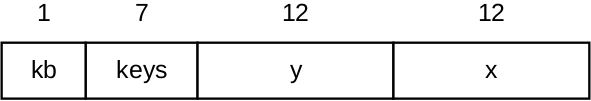
\includegraphics[width=.75\textwidth]{i/z}
	\caption{Format of the mouse register}
\end{figure}

\section{The SD-card (disk)}
SD-card are high-volume memory devices based on flash-store technology. They are typically
organized as individually accessible blocks of 1K bytes. The driver for the SD-card is contained in
module Kernel, which also handles allocation and reservation of blocks, here in analogy to rotating
disks still called sectors.
\begin{verbatim}
TYPE Sector = ARRAY SectorLength OF BYTE;
PROC GetSector(src: INT; VAR dst: Sector);
PROC PutSector(dst: INT; VAR src: Sector);
PROC AllocSector(hint: INT; VAR sec: INT);
PROC MarkSector(sec: INT);
PROC FreeSector(sec: INT);
\end{verbatim}

Data transfer is sequebtial and handled by procedures ReadSD and WriteSD by issuing
commands. These are for transmitting a block address, for receiving, and for sending a block of
data. Synchronous transmission of sequences of words follows the SPI standard, which uses 3
lines, one for data input, one for dats output, and one for the clock (see also Section 17.2.2). The
hardware interface contains a 32-bit register. The bit-rate is 8.3 MB/s.

\section{Serial asynchronous interface (RS 232)}
The RS-232 standard serves to transmit sequences of bytes over a data line asynchronously. This
implies that there is no separate clock line (see also Section 17.2.3). The hardware interface
contains a 10-bit register for the transmitter and one for the receiver. The data rate used here is
19200 bit/s. A byte is sent and received over the line by the following programs.
\begin{verbatim}
CONST data = -56; stat = -52; (*device register addresses*)
PROC Send(x: BYTE);
BEGIN
REPEAT UNTIL SYSTEM.BIT(stat, 1);
SYSTEM.PUT(data, x)
END Send;
PROC Rec(VAR x: BYTE);
BEGIN
REPEAT UNTIL SYSTEM.BIT(stat, 0);
SYSTEM.GET(data, x)
END Rec;
\end{verbatim}

These procedures are used in the driver module RS232 presented in Section 15.2. This module
itself is not used in the Oberon core, but it was instrumental in building the System on a host
computer and downloading it. It is characterized by a very simple interface.

\section{Serial communications controller (SCC)}
The interface of the driver for the network was taken over from the original design using a serial
communocations controller Zilog 8530. The implementation changed totally. It was designed by
Paul Reed for the wireless controller Nordic nRF24L01.
\begin{verbatim}
DEFINITION SCC;
TYPE Header =
RECORD valid: BOOL; dadr, sadr, typ: BYTE;
len: INT; (*of data following header*)
END ;
PROC Start(filter: BOOL);
PROC Send(VAR head: Header; buf: ARRAY OF BYTE);
PROC Available(): INT;
PROC ReceiveHead(VAR head: Header);
PROC Receive(VAR x: BYTE);
PROC Skip(m: INT);
PROC Stop;
END SCC.
\end{verbatim}
